\section{What was built around the mathematics}\label{sec:systems}

\subsection{A portfolio of executable instruments}

The Rust library implements field and curve arithmetic, generic and
specialised discrete-log methods, factor bases, Semaev oracles, SAT and
matrix engines, transfer experiments, external-CAS exporters, cost
accounting, curve identity and visual tools. The native C library
provides 64-bit reference groups and solvers, statistics, batched curve
arithmetic, preprocessing, bindings and distributed interfaces. These
64-bit primitives are research instruments; their parameter limit is
not a claim of cryptographic-size support.\src{C-README}\src{CA-README}

The broader library also contains symmetric ciphers, hash functions,
signature and nonce demonstrations, RSA and factoring routines,
pairings, zero-knowledge examples and post-quantum educational
implementations. Their presence documents capability breadth, not an
audited production cryptographic stack. For example, the current README
explicitly labels the STARK-like modules as educational, unaudited and
unsuitable for supporting a research security claim. This review does
not turn a module inventory into a security certification.

WDSat and the SQIsign repository are upstream solver/protocol forks and
integration resources; their imported histories are not independent
algorithmic contributions by this programme. The small standalone
ecbench repository is a companion entry point, while the principal
measuring implementation lives in crypto. Isogeny-labs supplies a
presentation layer. FPGA work includes field, point, step-unit and walker
models and simulation targets; the code inventory alone establishes no
measured silicon throughput. These distinctions prevent repository
proliferation from being counted as an equivalent number of new solvers.
\src{C-README}\src{CA-README}

The generic-group cost challenge adds a particularly useful boundary:
the solver receives opaque point tokens, while an oracle owns the real
coordinates and operation counter. This prevents an implementation from
silently doing unmetered point arithmetic. The same discipline motivates
the later explicit counters and sealed session records, although a
coordinate-aware IC study is a different computational model.
\src{COST}

\begin{figure}[htbp]
\centering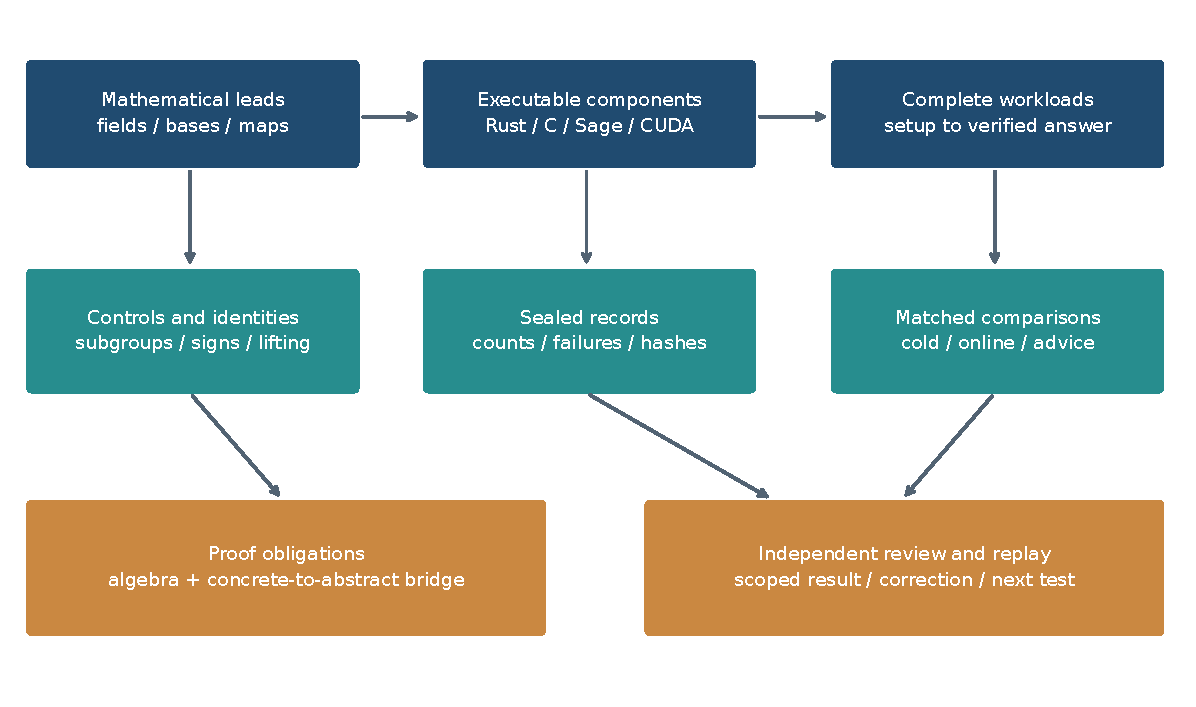
\includegraphics[width=\linewidth]{figures/research-map.pdf}
\caption{The implemented research stack and the distinct obligations
between a mathematical lead and an accepted complete-method claim.
Arrows are a conceptual workflow, not an assertion that every historical
study passed every gate. The catalogue and source register link the
concrete implementations behind each box.}
\end{figure}

\subsection{Research automation and preservation}

The autoresearcher separates coordinator, idea generator, executor,
reviewer, validator and red-team responsibilities. It implements
protocols, role policies, handoffs, immutable records, archive receipts,
corrections, claims, knowledge retrieval, runbooks and resource
coordination. This is research infrastructure whose aim is to prevent
an observation from being mistaken for an official scientific
transition.\src{AR-README}

The freshly parsed direct \texttt{ledger/goals/} files contain 72 goal
records: 36 draft, 26 active, six completed and four closed at budget.
These are literal stored status fields, not this paper's judgement of
scientific completion. Direct hypothesis files include 2,124 parsed
records; only 32 have exactly the literal status \texttt{supported}.
Other scoped and custom statuses are retained in the catalogue rather
than forced into a binary success metric. Legacy root records account
for why a whole-ledger wrapper count gives different totals.

The direct directories also contain 6,256 parsed handoffs, 2,634
proposals and 187 questions; missing status fields are common. These
counts measure coordination volume. Without deduplicated chains from
proposal to execution to independent review, they cannot yield a
meaningful ``research success rate''. The 24 safe-loader failures and
explicit correction records identify maintenance work rather than
silently disappearing from the denominator.

Cairn and associated runtime tools provide execution and custody
coordination. Their source and commits belong in an implementation
assessment, but this review does not infer actual rented compute,
financial spend, agent-hours or effective parallelism from their
existence. No verified consolidated bill or complete compute ledger
was available for that purpose.

\subsection{GPU rho, CPU arithmetic, and challenge operations}

The Blackwell release records an audited campaign build at 14.64
billion rho iterations per second on an RTX PRO 6000 Blackwell, with a
later best build at 15.88 billion. Its central mechanism is accelerated
binary-field arithmetic using the carry-less multiplication exposed by
the cited CUDA/PTX toolchain. Those are historical hardware-throughput
claims with provenance to the three central repositories; this review
does not remeasure them.\src{RHO-GPU}

The README also distinguishes the developed measurements from the
release snapshot's validation: the CPU client and planted solves were
run from that copy, while its Docker image and GPU modes were not yet
run there. The multi-card completion times are estimates from a work
model, not completed ECC2K-130 recoveries. Different documents quote
roughly 4.3 or five card-years under different builds and constants;
they must retain those assumptions rather than become a single measured
campaign duration.

The \texttt{ecc-challenges} service adds an operational evidence chain:
versioned raw uploads, namespaces, admission receipts, record validation,
point-relation checks, indexing and collision recovery. A durable upload
ACK is not the same as verified work. The v2 path checks curve membership
and $R=[a]G+[b]Q$ before index insertion, while reported trail lengths
still lack a work-verification model. Consequently point counts and
upload volume cannot honestly become percentage completion of a
challenge.\src{ECC-SERVICE}

An open C-library branch also identifies fruitless cycles in the GLV
walk and reports a corrective implementation. Its paired operation
ratios are 0.658 for $j=1728$ and 0.768 for $j=0$, with Bonferroni-adjusted
98.75\% intervals [0.630,0.688] and [0.753,0.784]. The author reports
432,000 correct toy solves across three builds. These are unmerged,
operation-count observations on 24--32-bit subgroups; the change does
not prove a new ECDLP hardness law. A stronger generic implementation
also changes the reference against which future IC must be measured.
\src{PR953}

\subsection{Quantum circuits and scheme construction}

The quantum point-addition work log studies reversible arithmetic scored
by average Toffoli count times peak qubits. Its recorded baseline is
1,739,149 average Toffolis, 1,434 qubits and score 2,493,939,666 over
9,024 validation shots. It also records truncation and reroll screening.
Those observations concern simulated circuit resources and finite
validation. Adaptive screening for a favourable Fiat--Shamir test set
does not prove correctness on every input. Upstream challenge progress
must not be credited as this programme's independent circuit advance,
and no fault-tolerant hardware ECDLP execution is demonstrated.
\src{QUANTUM}

EigenX is a separate constructive output: a Rust KEM/PKE research
implementation, wire formats, parameter sets, known-answer and hostile
input tests, and a Kani-chain/endomorphism design. Its current README
separates classical-optimised and quantum-hardened claim tiers after a
correction to earlier category language. Correct decapsulation at the
nominal parameter sizes establishes functionality, not the conjectured
security level. This is a scheme-construction research line and is not
evidence of an ordinary ECDLP break.\src{EIGEN}

Finally, \texttt{cryptologic-archives} preserves international standards
and historical cryptologic sources with claim and source catalogues.
It contributes provenance and contextual research, while its documentary
counts are not algebraic ECDLP experiments.\src{ARCHIVES}
